\section*{Introduction}
\addtocontents{toc}{\protect\setcounter{tocdepth}{0}}
\subsection*{Origins of group theory}
The mathematical field of group theory has its origins in the early 19th century.
At the time, mathematicians were investigating the solutions to polynomial equations.
That is, solutions to equations of the form
\[
	a_nx^n + a_{n-1}x^{n-1} + \ldots + a_0 = 0.
\]
Full solutions to polynomial equations of low degrees (i.e.\ $n \leq 4$) had already been formulated \cite{Riggs96}.
These include the familiar \emph{quadratic formula}, which has been known since antiquity.
The formula tells us that the solutions to a general quadratic equation $ax^2 + bx + c = 0$ are given by
\[
	x = \frac{-b\pm\sqrt{b^2-4ac}}{2a}.
\]
The full solutions to any cubic ($n=3$) or quartic ($n=4$) polynomial equation were also known.
These are given by the lesser-known Cardano's formula and Ferrari's method, respectively.
We say that a polynomial is \emph{solvable by radicals} if one can write all of its solutions in terms of its coefficients combined with the algebraic operations; addition, subtraction, multiplication, division, powers and radicals (i.e.\ $k^\text{th}$ roots).

In the 1830s, the mathematician Évariste Galois provided an elegant method to prove that a general polynomial of degree $n\geq 5$ is not solvable by radicals.
Galois understood that to every polynomial one could associate a \emph{Galois group}, a new mathematical object at the time.
The Galois group was the first object in a class of mathematical objects that we call \emph{groups} today.
We say that the pair $(G,\circ)$ is a group, where $G$ is a set and $\circ\colon G\times G\to G$ is a binary operation on $G$, when three conditions are satisfied:
\begin{itemize}
	\item Associativity: $g\circ (h\circ k) = (g\circ h)\circ k$ for all $g,h,k\in G$.
	\item Existence of an identity: there exists some $1_G\in G$ such that $1_G\circ g = g\circ 1_G = g$ for all $g\in G$.
	\item Existence of inverses: for every $g\in G$, there exists some $g^{-1}\in G$ such that $g\circ g^{-1}=g^{-1}\circ g = 1_G$.
\end{itemize}
Examples of groups that are likely familiar to the reader include $(\ZZ,+)$, the integers under addition, $(\RR^+,\times)$, the positive real numbers under multiplication, and $(\ZZ/n\ZZ,+)$, the integers modulo $n$ under addition.
Some geometric examples of groups are the \emph{dihedral groups}.
These groups are generated by the $m$ symmetries associated to the regular $m$-sided polygon (i.e.\ a polygon with all interior angles and all side lengths the same).
Then each dihedral group contains $2m$ elements ($m$ reflections and $m$ rotations) with the group operation of composition of reflections and rotations.
\begin{figure}[H]
	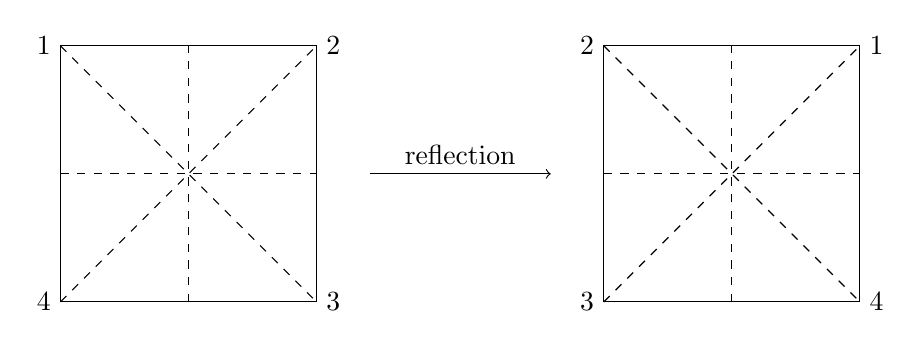
\begin{tikzpicture}[scale=1.15]
		\draw (-3,0)  +(45:2) node [right] {2} -- +(135:2) node [left] {1} -- +(225:2) node [left] {4} -- +(315:2) node [right] {3} -- cycle;
		\draw[dashed] (-3,-1.414) -- (-3,1.414);
		\draw[dashed] (-4.414,0) -- (1.414-3,0);
		\draw[dashed] (-4.414,1.414) -- (1.414-3,-1.414);
		\draw[dashed] (-4.414,-1.414) -- (1.414-3,1.414);
		\draw (3,0)  +(45:2) node [right] {1} -- +(135:2) node [left] {2} -- +(225:2) node [left] {3} -- +(315:2) node [right] {4} -- cycle;
		\draw[dashed] (-3+6,-1.414) -- (-3+6,1.414);
		\draw[dashed] (-4.414+6,0) -- (1.414-3+6,0);
		\draw[dashed] (-4.414+6,1.414) -- (1.414-3+6,-1.414);
		\draw[dashed] (-4.414+6,-1.414) -- (1.414-3+6,1.414);
		\draw[->] (-1,0) -- (1,0);
		\node [above] at (0,0) {{reflection}};
	\end{tikzpicture}
	\caption{The symmetries of a square and a reflection about the vertical line of symmetry.}
\end{figure}
This gives us an intuitive understanding of groups: they encode the symmetries of mathematical objects.

%%%%%%%%%%%%%%%%%%%%%%%%%%%%%%%%%%%%%%%%%%%%%%%%%%%%%%%%%%%%%%%%%%%%%%%%%%%%%%%%%%%%%%%%%%%%%%

\subsection*{What is representation theory?}
The study of groups yields insight into geometric objects.
The action of the dihedral group on the $m$-gon serves as example of a group acting on a geometric object.
More generally, we can consider the action of a group on some object.
Specifically, we say that a group $G$ \emph{acts} on a set $X$ if, for each $g\in G$, there is a map $\cdot\colon G\times X\to X$ satisfying $1_G\cdot x = x$ and $g\cdot (h\cdot x) = (gh)\cdot x$ for all $x\in X$.
Alternatively, one can view this as a group homomorphism $\rho\colon G\to \Sym(X)$, where $\Sym(X)$ is the symmetric group associated to $X$, i.e.\ the group of permutations of elements of $X$.

Now we linearise the setting above by requiring that $X=V$ is a \emph{vector space}.
Then we say that $G$ acts \emph{linearly} on $V$ if there exists a group homomorphism $\rho\colon G\to \GL(V)$.
We call $(V,\rho)$ a \emph{representation} of $G$, and $\rho$ is often suppresed from notation.
We see that $G$ acts on $V$ in the sense that $\rho(g)\colon V\to V$ is a linear invertible map on $V$.
We may denote $\rho(g)(v)$ by $g\cdot v$ as before.

Representation theory is concerned with understanding and classifying linear actions of groups.
The general situation of representation theory is as follows.
If the group $G$ acts on a vector space $V$, then we say that a vector subspace $W\subseteq V$ is a \emph{subrepresentation} of $V$ if it is invariant under the action of $G$.
A representation is called \emph{irreducible} if its only proper subrepresentation is the trivial representation $W=\{0\}$.
The primary goals of representation theory are finding all irreducible representations of $G$, and to decompose a given representation into its irreducible components.

We can think of irreducible representations as the building blocks of all other representations.
This is a common idea in mathematics, seen in other areas.
For instance, in number theory, the building blocks of integers are primes and, in group theory, the building blocks of groups are simple groups.

Writing a general representation in terms of irreducible components is not always possible.
We call a representation \emph{decomposable} if we can write it as the direct sum of irreducible representations.
A lot can be said about the case where the representation of a finite group is over a field whose characteristic not dividing the order of the group.
In this case, \emph{Maschke's theorem} tells us that these representations are always decomposable \cite{Lang02}.
In particular, complex representations of a finite group are always decomposable.

%%%%%%%%%%%%%%%%%%%%%%%%%%%%%%%%%%%%%%%%%%%%%%%%%%%%%%%%%%%%%%%%%%%%%%%%%%%%%%%%%%%%%%%%%%%%%%

\subsection*{Gelfand Pairs}
Henceforth, we assume some knowledge of abstract algebra from the reader.
Let $G$ be a finite group and $K\leq G$ a subgroup.
The pair $(G,K)$ is called a \emph{Gelfand pair} if the induced representation $\Ind_K^G \1$ is multiplicity-free.
Here $\1$ denotes the trivial ($1$-dimensional) complex representation of $K$, and multiplicity-free means that any irreducible representation appears in the decomposition of $\Ind_K^G \1$ at most once (up to isomorphism).

Gelfand pairs play an important role in representation theory \cites{Musili93}, analysis \cites{Koranyi80,Morel18}, combinatorics \cite{Bannai84}, number theory \cites{Gross91, Terras99} and probability \cites{CSST20, Diaconis88}.
One of our objectives is to give a detailed study of Gelfand pairs of finite groups.
A main theorem of this thesis is the following:
\begin{thm}(Gelfand's Trick)\label{theorem: Gelfands_Trick_intro}
	Let $G$ be a finite group and $K$ a subgroup of $G$.
	Suppose $\varphi\colon G\to G$ is an involutive anti-automorphism (i.e.\ a bijective anti-homomorphism) such that $K\varphi(x)K=KxK$ for all $x\in G$.
	Then $(G,K)$ is a Gelfand pair.
\end{thm}
The theorem above is proved using the \emph{Hecke algebra}.
There are multiple constructions of Hecke algebras in the  literature \cites{CMHL03,CSST20}.

%%%%%%%%%%%%%%%%%%%%%%%%%%%%%%%%%%%%%%%%%%%%%%%%%%%%%%%%%%%%%%%%%%%%%%%%%%%%%%%%%%%%%%%%%%%%%%

\subsection*{Types of Hecke algebras}
Another objective of this thesis is to present these a priori different Hecke algebras and resolve their apparent discrepancies.
For instance, one way to define the Hecke algebra is as a convolution algebra of $K$-bi-invariant complex-valued functions $f\colon G\to\CC$ on a group.
Another way to define the Hecke algebra is as the algebra generated by $n-1$ variables $T_1,\ldots T_{n-1}$ subject to a \emph{quadratic relation} $T_i^2 = (q-1)T_i + q$ and a \emph{braid relation}
\[
	\underbrace{T_iT_jT_i\ldots}_{m_{ij}\ \text{terms}}=\underbrace{T_jT_iT_j\ldots}_{m_{ij}\ \text{terms}}.
\]
Here $m_{ij}$ is the $ij^\text{th}$ entry in the \emph{Coxeter matrix} associated to the \emph{Weyl group} of $G$. The name `braid relation' is due to a method of visualising the \emph{symmetric group} $S_n$.
If $n$ is a positive integer then the group $S_n$ is the collection of bijections on the set $\{1,2,\ldots,n\}$ to itself, with the group operation of composing functions.
A natural method of visualising elements and multiplication in this group is via \emph{braid diagrams}.
For instance, if $\sigma = (1\ 2)(3\ 5\ 4)$ and $\pi = (1\ 2\ 4\ 6\ 5\ 3)$ are permutations in $S_6$ (written in cycle notation), then we may visualise these elements and their product $\pi\sigma = (1\ 4)(5\ 6)$ in the following manner:
\begin{figure}[H]
	\[
		\begin{pdiag}[1.5]{6}{2}
			\pdiagfill
			\pdiagmap{1}{2}
			\pdiagmap{2}{1}
			\pdiagmap{3}{5}
			\pdiagmap{4}{3}
			\pdiagmap{5}{4}
			\pdiagmap{6}{6}
			\pdiagname{$\sigma$}
			\pdiagendmap
			\pdiagmap{1}{2}
			\pdiagmap{2}{4}
			\pdiagmap{3}{1}
			\pdiagmap{4}{6}
			\pdiagmap{5}{3}
			\pdiagmap{6}{5}
			\pdiagname{$\pi$}
		\end{pdiag}
		=
		\begin{pdiag}[1.5]{6}{1}
			\pdiagfill
			\pdiagmap{1}{4}
			\pdiagmap{2}{2}
			\pdiagmap{3}{3}
			\pdiagmap{4}{1}
			\pdiagmap{5}{6}
			\pdiagmap{6}{5}
		\end{pdiag}
	\]
	\caption{A braid diagram visualising the multiplication $\pi\sigma = (1\ 4)(5\ 6)$.}
\end{figure}

%%%%%%%%%%%%%%%%%%%%%%%%%%%%%%%%%%%%%%%%%%%%%%%%%%%%%%%%%%%%%%%%%%%%%%%%%%%%%%%%%%%%%%%%%%%%%%

\subsection*{Why study Hecke algebras?}
The Hecke algebra arises naturally when one wishes to compute certain irreducible representations of a group \cite{Williamson21,CMHL03}.
Consider a finite group $G$ and a normal subgroup $N\triangleleft G$.
If $G$ acts linearly on a vector space $V$ (i.e.\ $V$ is a representation of $G$), then there is a natural action of $G$ on the subrepresentation $V^N$, the space of vectors in $V$ that are fixed by $N$.
Under this action, $N$ will clearly act trivially on $V^N$.
This yields a representation of the quotient group $G/N$.
After some representation theoretic arguments, one arrives at the conclusion that
\[
	\left\{\begin{array}{c}
		\text{Irreducible representations} \\
		\text{of $G$ with $N$-fixed vectors}
	\end{array}\right\}
	\stackrel{1:1}{\longleftrightarrow}
	\left\{\begin{array}{c}
		\text{Irreducible representations} \\
		\text{of $G/N$}
	\end{array}\right\}.
\]
It is a straightforward exercise that a complex representation of the group $G/N$ is the same as a representation of the algebra $\CC[G/N]$, the \emph{group algebra} of $G/N$.

What happens when we do not require a normal subgroup of $G$? Consider an arbitrary subgroup $K$ of a finite group $G$.
Now $G/K$ is no longer necessarily a group, so $G/K$ and $\CC[G/K]$ no longer necessarily make sense.
We ask ourselves: what acts on $V^K$?
The action of $G$ on $V$ is not well-defined on $V^K$ since $K$ is no longer normal.
It is not obvious how we could study irreducible $G$-representations with $K$-fixed vectors.
We are able to salvage the situation with the help of the Hecke algebra.

For $g\in G$, define the Hecke operator $[KgK] := \frac{1}{|K|}\sum_{x\in KgK} x\in\CC[G]$, which acts on $V^K$ by
\[
	[KgK]\cdot v := \frac{1}{|K|}\sum_{x\in KgK} x\cdot v.
\]
Now define the Hecke algebra $\calH(G,K)$ to be the space of functions $f\colon G\to\CC$ that are constant on $K$-double cosets.
The indicator functions $\chi_{KgK}$ form a basis of this space and we can uniquely associate the indicator functions $\chi_{KgK}$ to the Hecke operators $[KgK]$.
We see that, through the Hecke operators, we have defined an action of $\calH(G,K)$ on $V^K$.
This answers our question of what acts on $V^K$.
Through another representation-theoretic exercise, one can conclude that
\[
	\left\{\begin{array}{c}
		\text{Irreducible representations} \\
		\text{of $G$ with $K$-fixed vectors}
	\end{array}\right\}
	\stackrel{1:1}{\longleftrightarrow}
	\left\{\begin{array}{c}
		\text{Irreducible representations} \\
		\text{of $\calH(G,K)$}
	\end{array}\right\}.
\]
An immediate example of the utility of this result is as follows. It is easy to show that if $\calH(G,K)$ is commutative, then all of its irreducible finite-dimensional representations are one-dimensional \cite{Etingof11}.
The commutativity of the Hecke algebra turns out to be an important property which will be investigated throughout this thesis.

%%%%%%%%%%%%%%%%%%%%%%%%%%%%%%%%%%%%%%%%%%%%%%%%%%%%%%%%%%%%%%%%%%%%%%%%%%%%%%%%%%%%%%%%%%%%%%

\subsection*{Contents of this thesis}
In Chapter \ref{Chapter1}, we begin our study of the Hecke algebra.
First, we investigate the convolution algebra of all complex-valued functions on $G$ and its ideal of $K$-right-invariant complex-valued functions.
This is followed by results describing the relationship between the induced representation and its associated Hecke algebra.
We use these results to prove Theorem \ref{theorem: Gelfands_Trick_intro}.
This allows us to write down simple proofs that $\Ind_K^G \1$ is multiplicity-free for certain choices of $G$ and $K$.
Namely, $(G,K)$ with $G$ commutative, $(G,K)$ with $[G\! :\! K]=2$, $(S_{n+m}, S_n\times S_m)$, and $(O_{n+1}(\FF_q), O_n(\FF_q))$ for $q$ odd.

In Chapter \ref{Chapter2}, we generalise the discussion of Chapter 1 to the case of a non-trivial \emph{character} $\sigma\colon K\to\CC^\times$.
Here our goal is to obtain a twisted analogue of Theorem \ref{theorem: Gelfands_Trick_intro}.
To this end, we describe the basis of the Hecke algebra using the idea of \emph{relevant orbits}.
We state and prove the generalisation of Theorem \ref{theorem: Gelfands_Trick_intro}.
We apply the new theorem to a particular representation, the \emph{Gelfand--Graev representation} of $\GL_n(\FF_q)$, to show that it is multiplicity-free.

In Chapter \ref{Chapter3}, we investigate the Hecke algebra of Chapter \ref{Chapter1} under the particular choice of $G=\SL_n(\FF_q)$ and $K=B(\FF_q)$, the \emph{Borel subgroup} of $G$, i.e.\ the subgroup of upper-triangular matrices.
The \emph{Weyl group} associated to $G$ is introduced and shown to be isomorphic to $S_n$.
Next, we perform some elementary matrix calculations which yields the surprising result above: the Hecke algebra may be written in terms of $n-1$ generators subject to the quadratic relation and the braid relations associated to $W$.
This leads to a concluding discussion of Hecke algebras generated by any finite \emph{Coxeter group}.

In Chapter \ref{Chapter4}, we generalise the results of earlier chapters to the case where $G$ is no longer finite, but instead a locally compact topological group.
This allows for an extension of the theory we have developed to more general groups and their Hecke algebras.
To do this, we discuss how one can impose a topological structure on a group and supply examples to give some intuition for these types of groups.
To define Hecke algebras of these groups, we require some measure theory.
In particular, the convolution product on the Hecke algebra is defined in terms of an integral with respect to the \emph{Haar measure}.
We spend some time developing the theory of Haar measures for this purpose.
We conclude with a discussion of how to recover the Hecke algebra of a finite group from this new definition.
In this chapter, we shall denote the Hecke algebra by $C_c(K\backslash G/K)$ to emphasise the non-finiteness of $G$.

In Chapter \ref{Chapter5}, we take a look at some specific Hecke algebras of locally compact topological groups.
In particular, we restrict our attention to the general linear group over a non-archimedian local field $k$ and its ring of integers $\calO$.
We look at the \emph{Spherical Hecke algebra}, formed when one considers $G=\GL_n(k)$ and $K=K^\circ := \GL_n(\calO)$, and the \emph{Iwahori--Hecke algebra}, formed when one considers $G=\GL_n(\calO)$ and $K=I$, the \emph{Iwahori subgroup}.
In order to investigate these algebras, we must develop an understanding of these fields.
We detail their definition, classification and structure.

The contents of this thesis may be visualised with the following diagram.
\begin{figure}[H]
	% https://q.uiver.app/?q=WzAsNixbMSwwLCJcXGNhbEgoRyxLKSJdLFsyLDAsIkNfYyhLXFxiYWNrc2xhc2ggRy9LKSJdLFszLDAsIkNfYyhJXFxiYWNrc2xhc2ggRy9JKSJdLFswLDAsIlxcY2FsSChHLEssXFxzaWdtYSkiXSxbMSwxLCJcXGNhbEhfcShXLFMpIl0sWzIsMSwiQ19jKEteXFxjaXJjXFxiYWNrc2xhc2ggRy9LXlxcY2lyYykiXSxbMSw1LCJLPUteXFxjaXJjIl0sWzEsMCwiR1xcIFxcdGV4dHtmaW5pdGV9IiwyXSxbMSwyLCJLPUkiXSxbMCw0LCJHXFwgXFx0ZXh0e0xpZSB0eXBlfSJdLFszLDAsIlxcc2lnbWE9XFwxIl1d
	\[
		\begin{tikzcd}
			{\overset{\text{Ch.\ \ref{Chapter2}}}{\calH(G,K,\sigma)}} & {\overset{\text{Ch.\ \ref{Chapter1}}}{\calH(G,K)}} & {\overset{\text{Ch.\ \ref{Chapter4}}}{C_c(K\backslash G/K)}} & {\overset{\text{Ch.\ \ref{Chapter5}}}{C_c(I\backslash G/I)}} \\
			& {\underset{\text{Ch.\ \ref{Chapter3}}}{\calH_q(W,S)}} & {\underset{\text{Ch.\ \ref{Chapter5}}}{C_c(K^\circ\backslash G/K^\circ)}}
			\arrow["{K=K^\circ}", from=1-3, to=2-3]
			\arrow["{G\ \text{finite}}"', from=1-3, to=1-2]
			\arrow["{K=I}", from=1-3, to=1-4]
			\arrow["{\substack{G\ \text{Lie type}\\ \text{over}\ \FF_q}}", from=1-2, to=2-2]
			\arrow["{\sigma=\1}", from=1-1, to=1-2]
		\end{tikzcd}
	\]
	\caption{The relationship diagram of this thesis.}
\end{figure}

%%%%%%%%%%%%%%%%%%%%%%%%%%%%%%%%%%%%%%%%%%%%%%%%%%%%%%%%%%%%%%%%%%%%%%%%%%%%%%%%%%%%%%%%%%%%%%

\subsection*{Directions for future research}
We assume the reader is familiar with the contents of this thesis.
The modern study of Hecke algebras is largely focused on the \emph{Iwahori--Hecke algebra}, which is also known as the \emph{affine Hecke algebra}.
This algebra is central to the study of representations of \emph{reductive groups} over non-archimedian local fields (e.g.\ groups such as $\GL_n$, $\SL_n$, $\Sp_{2n}$ over fields such as $\QQ_p$ or $\FF_q(\!(t)\!)$).

Some topics relevant to the Iwahori--Hecke algebra include \emph{Bernstein's presentation}, the \emph{Iwahori--Matsumoto presentation} and the \emph{Satake isomorphism} \cite{HKP}.
Properties of the Iwahori--Hecke algebra such as these presentations may be viewed as a consequence of the \emph{universal unramified principal series module}, which we now describe.

Fix a ``nice'' (i.e.\ split and connected) reductive group $G$ (e.g.\ $\SL_n$) over a non-archimedian local field $k$ with ring of integers $\calO$.
Then write $A$ to mean a \emph{split maximal torus} of $G$ and write $N$ to mean the \emph{unipotent radical} of a Borel subgroup of $G$ that contains $A$.
Also recall $I$ is the Iwahori subgroup of $G$ given in Chapter \ref{Chapter5}.

The universal unramified principal series module $M$ is given by $C_c(A(\calO)N\backslash G/I)$.
It is a right module over the Iwahori--Hecke algebra under convolution.
Furthermore, a basis of the Iwahori--Hecke algebra is parameterised by the \emph{affine Weyl group} $\widetilde{W}$.
We may write $\widetilde{W} \cong W \ltimes \Lambda^\vee$, where $\Lambda^\vee$ is the \emph{coroot lattice} of $G$.
Then $\CC[\Lambda^\vee]$ is the corresponding group algebra over $\CC$.
Then $M$ is also a left module over $\CC[\Lambda^\vee]$.

\newpage
\addtocontents{toc}{\protect\setcounter{tocdepth}{2}}
%%%%%%%%%%%%%%%%%%%%%%%%%%%%%%%%%%%%%%%%%%%%%%%%%%%%%%%%%%%%%%%%%%%%%%%%%%%%%%%